\documentclass[11pt]{article}
% Language setting
% Replace `english' with e.g. `spanish' to change the document language
\usepackage[english]{babel}
\usepackage[page,header]{appendix}
\usepackage{titletoc}
\usepackage{subcaption}
% Set page size and margins
% Replace `letterpaper' with `a4paper' for UK/EU standard size
\usepackage[letterpaper,top=2cm,bottom=2cm,left=3cm,right=3cm,marginparwidth=1.75cm]{geometry}

% Useful packages
\usepackage[colorlinks=true, allcolors=blue]{hyperref}
\usepackage{amsmath}
\usepackage{amssymb}
\usepackage{bm}
\usepackage{graphicx}
\usepackage{setspace}
\usepackage{color}
\usepackage{enumitem}
\usepackage{cancel}
\usepackage{lineno}
\usepackage{authblk}
%\usepackage{siunitx}  % RES: when I try to compile, it stumbles over siunitx.sty

\usepackage{mathtools}
\usepackage[font=small,skip=0pt]{caption}

\newcommand{\comment}{\textcolor{blue}}

%Useful new commands
\newcommand{\A}{\mathbf{A}}
\newcommand{\Abar}{\overline\A}
\newcommand{\w}{\mathbf{w}}
\newcommand{\wbar}{\overline\w}
\newcommand{\vbar}{\overline\bbv}

%% Commented out so that Robin can compile:
% Chrissy bibliography:
% \usepackage[
%     citestyle=authoryear, 
%     uniquelist=false,
%     uniquename=false,
%     natbib,
%     backend=biber,
%     bibstyle=apa,
%     ]{biblatex}
% \addbibresource{hernandez_library.bib}

\title{luckieR: an R package for calculating and decomposing distributions of luck in life histories}
\author[1]{Stephen P. Ellner}
\author[2]{Christina M. Hern\'andez\thanks{Corresponding author. Email: cmhernan@odu.edu}}
\author[3]{Robin E. Snyder}
% Authors currently alphabetical

\affil[1]{Cornell University, Department of Ecology and Evolutionary Biology, Ithaca, NY, USA}
\affil[2]{Old Dominion University, Department of Biological Sciences, Norfolk, VA, USA}
\affil[3]{Case Western Reserve University, Department of Biology, Cleveland, OH, USA}

\begin{document}
\maketitle

\noindent For submission at \textit{Methods in Ecology and Evolution} as an \textit{Application} paper.

\paragraph{Running title} luckieR package

\paragraph{Acknowledgements} ADD FUNDING INFORMATION

\paragraph{Author Contributions} All authors contributed R functions to the package. CMH built and submitted the package to CRAN. All authors wrote and revised the manuscript text.

\paragraph{Data availability statement} The R package \texttt{luckieR} is available on CRAN and at Github (\url{https://github.com/chrissy3815/luckieR}). \textcolor{red}{REF VIGNETTES?} All code files required to repeat the worked examples are archived at Zenodo (\textcolor{red}{ADD LINK WHEN RELEVANT}). 
\paragraph{Word count} Abstract: \textless 350, Main text: \textless 4000\\
\textbf{Figures} Main text: 2 figures, 1 table\\

% Journal scope statement for MEE: 
% We present a mathematical decomposition of variance in population growth rate into contributions from variation in vital rates and population structure. We present analytical expressions, the resulting theoretical expectations, and a simulation approach. To demonstrate interpretation of results, we include case studies. Our methods are broadly relevant to population ecology.

\newpage

\doublespacing
\begin{linenumbers}

\section*{Abstract}
1. Luck is important and a robust set of tools have been introduced across multiple papers. These tools do X, Y, Z.

\noindent 2. Here, we introduce an R package, luckieR, that brings together many of the tools for calculating luck metrics. The generalized software available through luckieR is a user-friendly toolkit for calculating a variety of 

\noindent 3. We demonstrate the utility of the package and its functions for ecological investigations through two worked examples. First, we demonstrate the insight about variation among individuals in life history outcomes that can be gained from a single matrix model, using an example from the COMADRE animal matrix population model database. To highlight the more complex analyses that are possible with our software, we present a luck decomposition analysis of an IPM for a grass-endophyte experiment that includes both trait and environmental variation.

\noindent 4. In conclusion, luckieR facilitates sophisticated analyses of variation among individuals in a population in their life history outcomes such as age of maturity, lifespan, and lifetime reproductive output. The package is open source and available on CRAN. As analyses of luck in life histories continue to be developed, luckieR will provide a centralized resource for software to perform those calculations.

\noindent \textbf{Data/code for peer review statement:} An anonymized version of the code has been provided as a zip file containing \textcolor{red}{NUMBER} R script files. We have also provided an anonymized README.txt file, and two CSV data files. \textcolor{red}{Will need to look into how to anonymize the package?}

\noindent \textbf{Keywords:} lifetime reproductive output, matrix population models, \textcolor{red}{OTHERS}

\newpage
\section{Introduction}

\section{Package Overview}
Different papers use different headers for this section: Implementation, Modeling Approach, etc. We can change section names or number of sections as needed.

\subsection{Chrissy's questions about software dev}
\begin{enumerate}
	\item Robin's functions have different options for different cases (NoEnv, PostBreeding, PostBreedingNoEnv). Is it worth creating a wrapper that has input variables that allow users to select pre- vs. post-breeding and environment vs no environment? Chrissy is offering to do that if it's desirable.
	\item Is it possible to change ``Def3" to something more
          intuitive? \comment{RES: yes, I'll add that to my to-do list.}
\end{enumerate}

\section{Example Applications}

As an example, consider a size-structured model for \emph{Elymus
  villosus}, a perennial grass, for individuals with and without
endophytes~\citep{2024:fowle.ziegl.whitn.ea}.  The model is based on
data from a long-term symbiont removal experiment at Lilly-Dickey
Woods in Indiana, USA~\citep{2023:mille.fowle.ziegl.ea} and contains
transition matrices for 13 years.  One question we may wish to ask is
how certain we are of an individual's endophyte status based on their
lifetime reproductive output (LRO).  Fig.~\ref{fig:ELRIfigs} top left,
is generated with \texttt{probTraitCondLRO} and shows that for this
species, not having endophytes produces higher LRO, but even if we
observe an individual with 6 offspring (which is well into the 90th
percentile), we can't be very confident that that individual lacked
endophytes.  For more details on the math behind this calculation,
see~\cite{2018:snyde.ellne,2024:snyde.ellne}.

Alternatively, we may wish to focus on what forms of luck are most
important and at what ages.  If we partition the variance in LRO into
a within-endophyte-status contribution and a between-endophyte-status
contribution, we can think of the within-endophyte-status contribution
as the contribution of luck~\citep{2018:snyde.ellne}.  We can further
partition that luck contribution into contributions from individual
demographic transitions at different ages.  Did you survive from age 2
to age 3 and how much does knowing the outcome reduce the overall
variance?  If you lived, how much did you grow or shrink and how much
does knowing the outcome reduce the overall variance?  And so forth.
The amount that knowing the outcome of each of these demographic
transitions reduces the overall variance is the contribution that
transition makes.

Fig.~\ref{fig:ELRIfigs} top right shows that early survival luck is key,
and this makes sense: if you die young, it doesn't matter how lucky
you would have been later.  We also see that growing quickly at ages 2
and 3 is important.  Survival rises rapidly with size for this
species, so this too, makes sense.  For the mathematical details
behind this calculation, see~\cite{2024:snyde.ellne}.

As a final example, let us plot survival fraction and average size vs
age for those destined to have at least one offspring and for those
who will never have any offspring, as a way of understanding what is
different about successful breeders.  To do this, we need to calculate
the survival/growth transition matrices conditional on having at least
one offspring.  Fig.~\ref{fig:ELRIfigs} bottom shows that that most of those
who never breed fail because they do not survive the seedling stage
(age 0), and of those that do, those that never breed do not grow as
large as those who do.  Survival increases sharply with size for this
species, so growing large quickly increases survival, not just
fecundity.  For the mathematical details behind this calculation,
see~\cite{2018:snyde.ellne}.

\begin{figure}[htb]
  \centering
  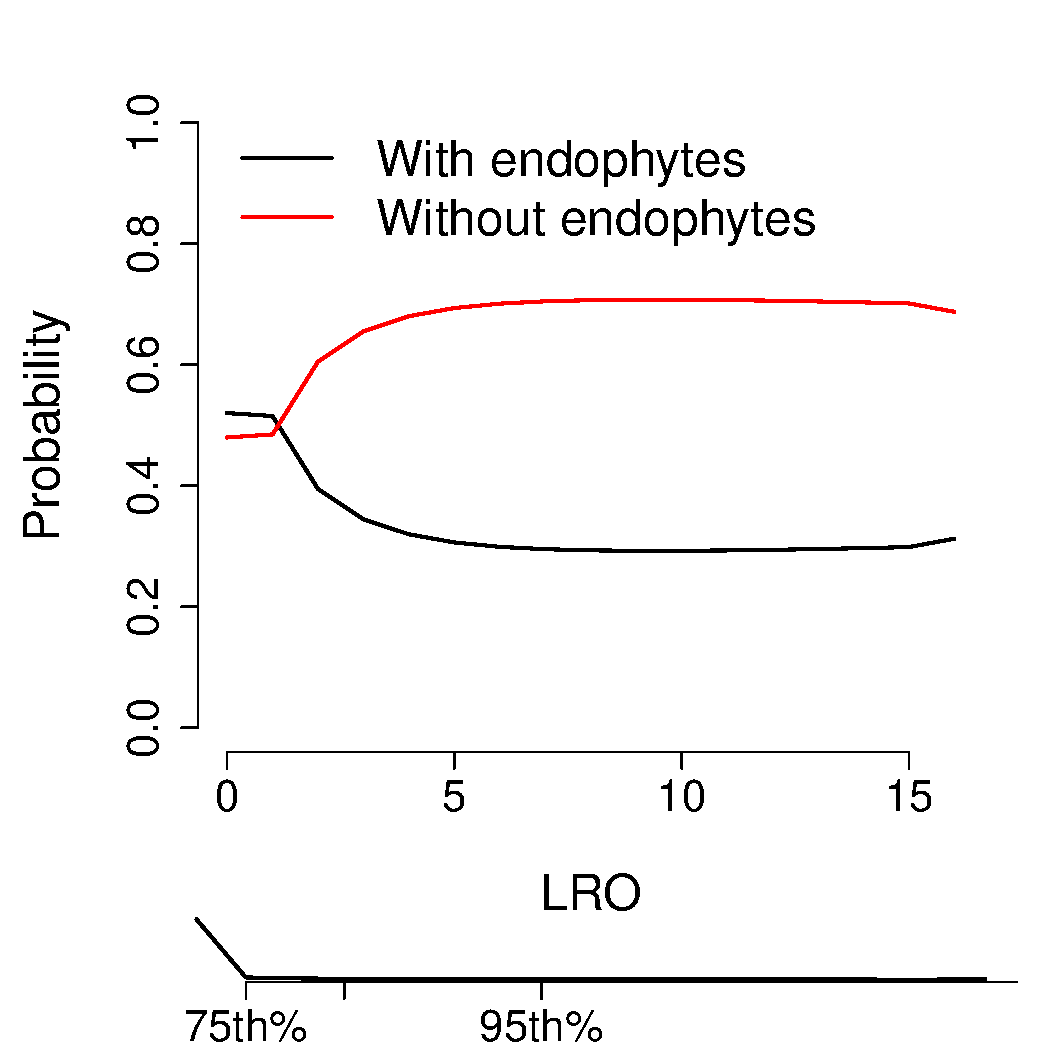
\includegraphics[width=0.47\linewidth]{probXCondR}
  \hspace{3mm}
  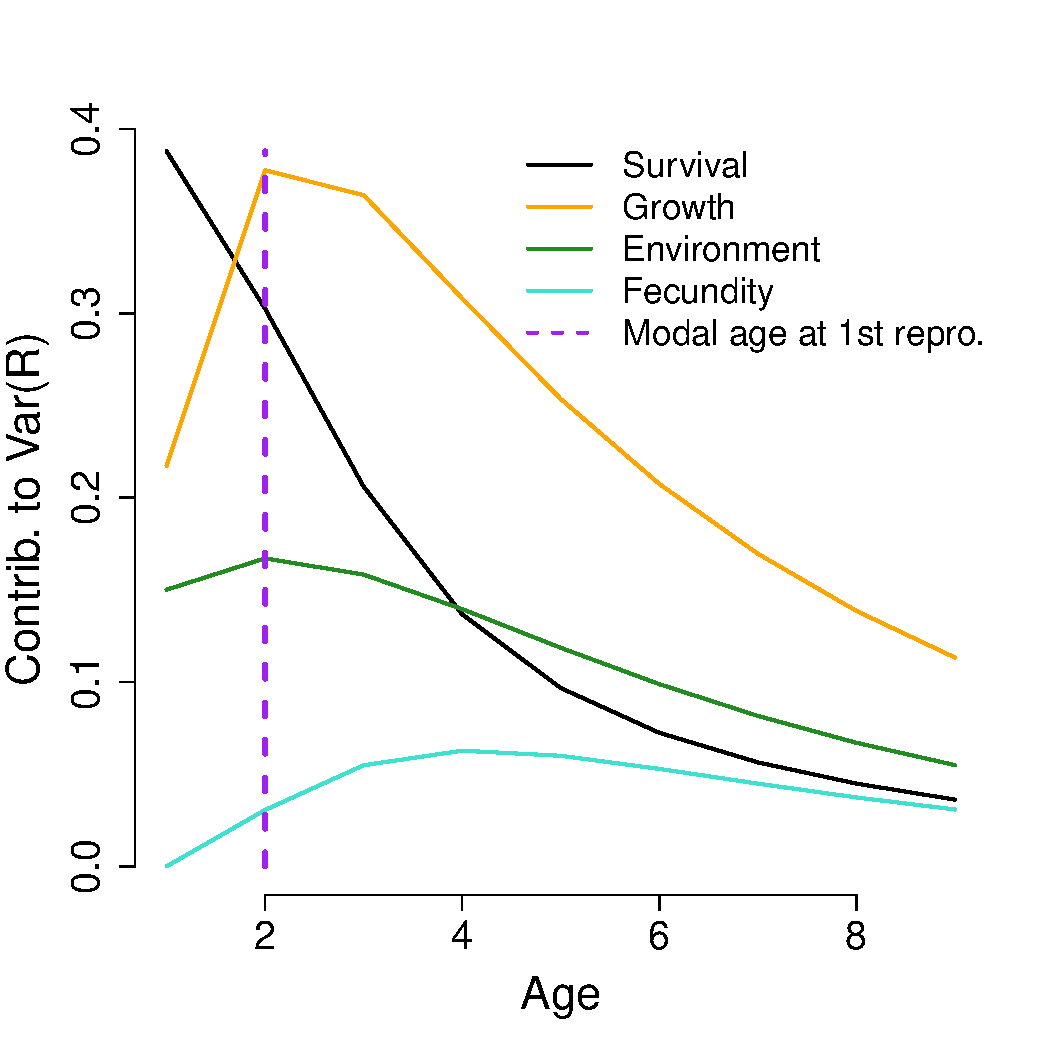
\includegraphics[width=0.47\linewidth]{luckTrajecELRI}

  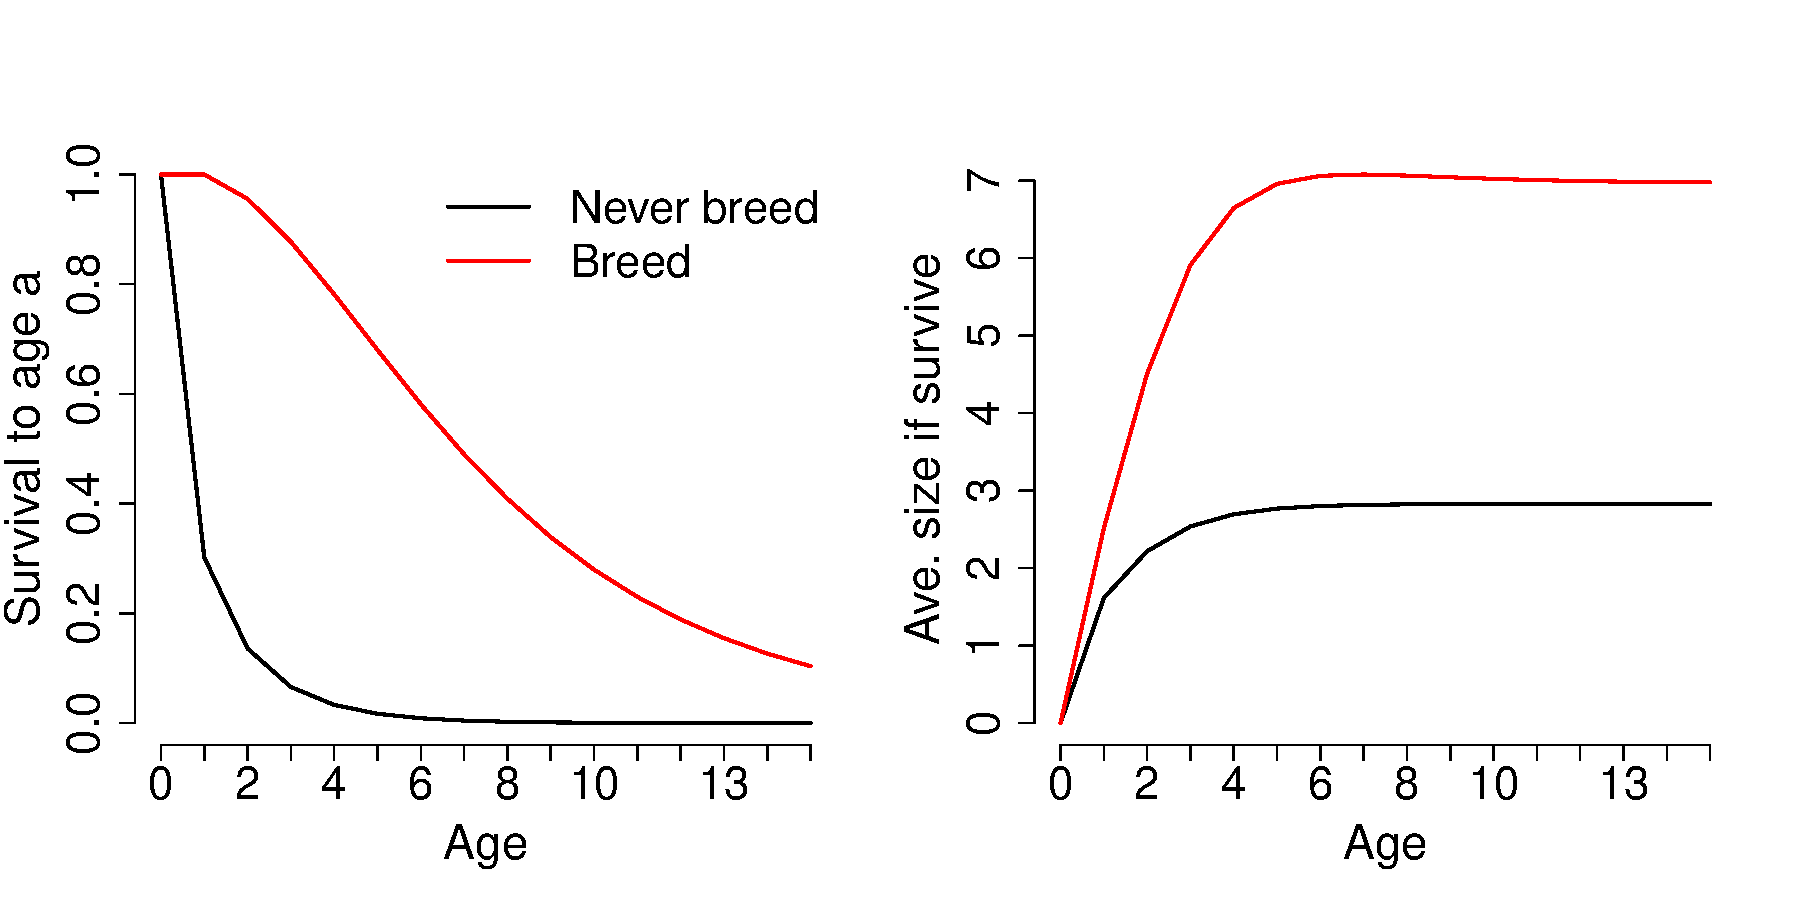
\includegraphics[width=\linewidth]{condKernelPlots}
  \caption{Top left: The probability that an individual is
    endophyte-positive (black) or -negative (red) given their LRO.
    Axis tics are at the 75th, 90th, 95th percentiles, and the plot
    extends to the 99th percentile.  Top right: Contributions to
    $\var(R)$ as a function of age for endophyte-positive individuals.
    The plot extends to the age by which an individual is 95\% likely
    to have died, while the dashed purpble line shows the modal age at
    first reproduction.  Bottom: Survival and average size vs age for
    endophyte-positive individuals with and without offspring.}
  \label{fig:ELRIfigs}
\end{figure}

\section{Discussion}


\newpage
\begin{table}[ptb]
  \renewcommand{\arraystretch}{1.2}
  \caption{List of functions included in luckieR vXXXX. We could add references to where the more-complete math is introduced? Or we could add usage details?} 
  \label{tab:notation}
  \begin{center}
    \small
    \vspace{-0.2in}
    \begin{tabular}{lp{0.1cm}p{10.5cm}}
      \hline
      \textbf{Function name}& & \textbf{Short description}  \\
      \hline
       \multicolumn{3}{l}{\textbf{Basic calculations}} \\[-3pt]
      calcDistLRO &&  and friends: NoEnv, PostBreeding, PostBreedingNoEnv \\[6pt]
      \multicolumn{3}{l}{\textbf{Functions for calculating conditional distributions}}\\[-3pt]
      calcDistOffspringCohort && Calculates the distribution of offspring types in a cohort produced by the stable population distribution. \\
      calcMoments &&   \\
      distLifespanCondR2 && And NoEnv, PostBreeding, and PostBreedingNoEnv versions. \\
      firstBreed &&   \\
      flatten &&   \\
      fundamental\_matrix &&  change to camel case, I think? \\
      makeCondFailureKernel &&  \\
      makeCondKernel &&  \\
      makeM &&  \\
      makeMCondLROThreshold && And version for PostBreeding \\
      makePCondBreedDef3 && This does not have the most intuitive name \\
      makePDef3 && Is it possible to change ``Def3" to something descriptive? \\
      make\_AxT && \\
      meanConditionalLifespan && \\
      meanConditionalTimes && \\
      meanLRO && \\
      meanLifespan && \\
      mk\_B && change to ``make" to match other functions? and change to camel case. \\
      mk\_BPostBreeding && same comment as line above \\
      p\_xT && \\
      partitionVarSkewnessEnvVar && and friends: partitionVarSkewnessEnvVarAndTraits, partitionVarSkewnessEnvVarPostBreeding, partitionVarSkewnessNoEnvVar, partitionVarSkewnessNoEnvVarPostBreeding \\
      popMeanVar && \\
      probRepro && \\
      probTraitCondLRO && and friends: NoEnv, PostBreeding, PostBreedingNoEnv \\
      skewLRO && \\
      skewLifespan && \\
      stable\_dist && Change to camel case \\
      traitAve && Change to ``mean"? \\
      traitMu3 && \\
      traitVar && \\
      unfold && Does this function need to be exported? \\
      unvec && Does this function need to be exported? \\
      varConditionalLifespan && \\
      varConditionalTimes && \\
      varLRO && \\
      varLifespan && \\
      vec && \\
      \hline
    \end{tabular}
   \normalsize
  \end{center}
  \renewcommand{\arraystretch}{1}
\end{table}

\end{linenumbers}

%\printbibliography

\end{document}
